\section{Kernel Discriminant Analysis against Masking}


\subsection{Linear Discriminant Analysis}

%\begin{frame}
%\frametitle{Contents}
%\begin{itemize}
%\item \important{Introduction to LDA: as a classifier, and as a feature extractor}
%\item Introduction to masking countermeasure and Kernel Discriminant Analysis as a feature extractor
%\item Motivations to apply deep learning techniques
%\item Convolutional Neural Networks and Data Augmentation to attack jitter-based countermeasure
%\end{itemize}
%\end{frame}



\begin{frame}
\frametitle{Model-based SNR and Fisher's Criterion}
\begin{block}{Signal-to-Noise Ratio (SNR)}
\begin{itemize}
\item Independent Noise Assumption: $\vaLeakVec = \varphi(\sensRandVar)+\vec{B}$

\item $\mmmXclass= \esperEst[\given{\vaLeakVec}{\sensRandVar = \sensVarGenValue}] = \frac{1}{\nbTracesPerClass}\sum_{i\colon \sensVar_i=\sensVarGenValue} \vLeakVec_i $ sample mean per class ($\approx \varphi(\sensRandVar)$)
\item $\varXclass = \varEst(\given{\vaLeakVec}{\sensRandVar = \sensVarGenValue}) = \frac{1}{\nbTracesPerClass-1}\sum_{i\colon \sensVar_i=\sensVarGenValue} (\vLeakVec_i - \mmmXclass)^2 $ sample variance per class ($\approx \mathrm{var}(\vec{B})$) 
\item \begin{equation*}\mathrm{SNR}(t) = \frac{\varEst(\mmmXclass[Z](t))}{\esperEst[\varXclass[Z](t)]} \qquad \textcolor{grey}{\frac{\text{\emph{variance inter-class}}}{\text{\emph{variance intra-class}}}} \end{equation*}
\end{itemize}
\end{block}

\begin{block}{Fisher's Criterion for Linear Dimensionality Reduction}

\begin{itemize}
\item $\SB = \sum_{\sensVarGenValue\in\sensVarSet}\nbTracesPerClass(\mmmXclass-\mmmX)(\mmmXclass-\mmmX)^\intercal $ (inter-class scatter matrix)
\item $\SW = \sum_{\sensVarGenValue\in\sensVarSet}\sum_{i=1\colon \sensVar_i=\sensVarGenValue}(\vLeakVec_i-\mmmXclass)(\vLeakVec_i-\mmmXclass)^\intercal$ (intra-class scatter matrix)
\item Fisher's criterion
 \begin{equation}\label{eq:LDA}
\hat{ \AAlpha}=\mathrm{argmax}_{\AAlpha} \frac{\AAlpha^\intercal \SB \AAlpha}{\AAlpha^\intercal \SW \AAlpha} \mbox{ ,}
 \end{equation}
\end{itemize}

\end{block}
\end{frame}

\begin{frame}
\frametitle{LDA: an optimal binary linear classifier}
\begin{columns}
\begin{column}{.5\linewidth}
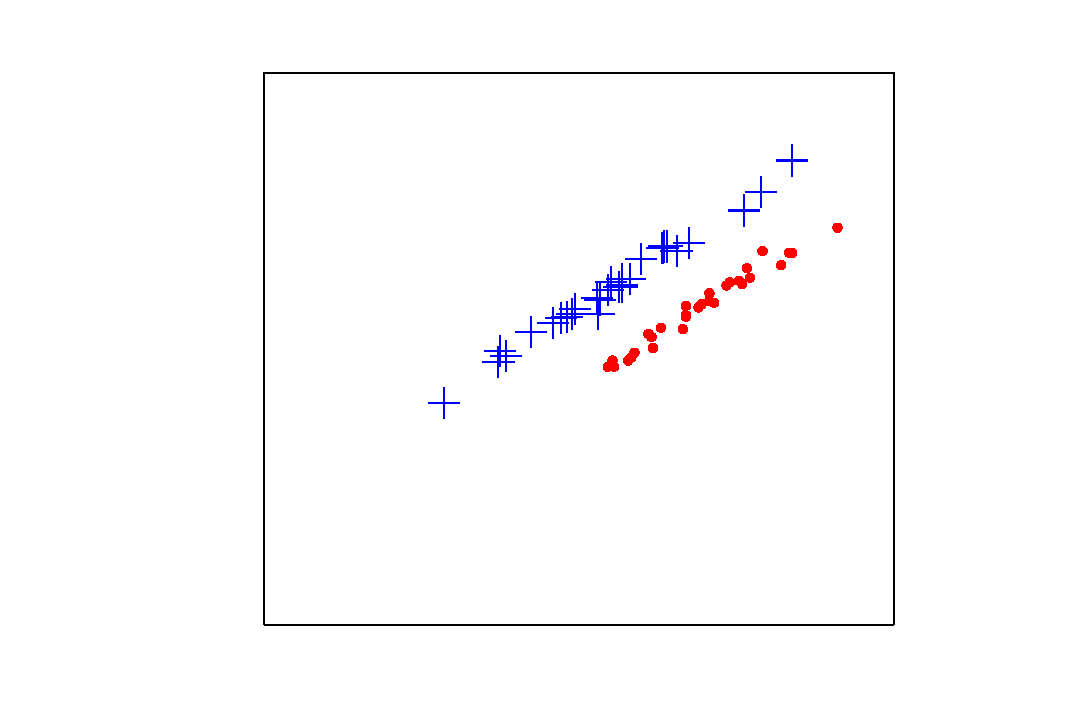
\includegraphics[width=\textwidth]{figures/dataNoProjection.pdf} 
\end{column}
\begin{column}{.6\linewidth}
\begin{itemize}
\item Classify data $\vLeakVec$ into 2 classes $\sensVarSet = \{\sensVarValue{1}, \sensVarValue{2}\}$
\item Generative model: $\pdf_{\given{\vaLeakVec}{\sensRandVar = \sensVarValue{j}}}(\vLeakVec)$, $\pdf_{\sensRandVar}(\sensVarValue{j})$ and $\pdf_{\vaLeakVec}(\vLeakVec)$
\item Posterior probabilities (via Bayes' theorem), then classify through the \emph{log-likelihood ratio}: $a = \log\left[\frac{\prob(\given{\sensVarValue{1}}{\vLeakVec})}{\prob(\given{\sensVarValue{2}}{\vLeakVec})}\right]]$ (boundary surface $a=0$)
\end{itemize}
\end{column}
\end{columns}

\begin{itemize}
\item Two assumptions about class-conditional densities: 
\begin{itemize}
\item Gaussian distributions with parameters $\mu_j, \Sigma_j$
\item Homoscedasticity: $\Sigma_j=\Sigma$ for all $j$
\end{itemize}
\item $\Rightarrow a = \vec{w}^\intercal \vLeakVec + w_0$ (linear decision boundary, $\vec{w}$ and $w_0$ functions of $\Sigma, \mu_j$)
\end{itemize}

\end{frame}

\begin{frame}
\frametitle{LDA and Fisher's Discriminant}
\begin{columns}
\begin{column}{.5\linewidth}
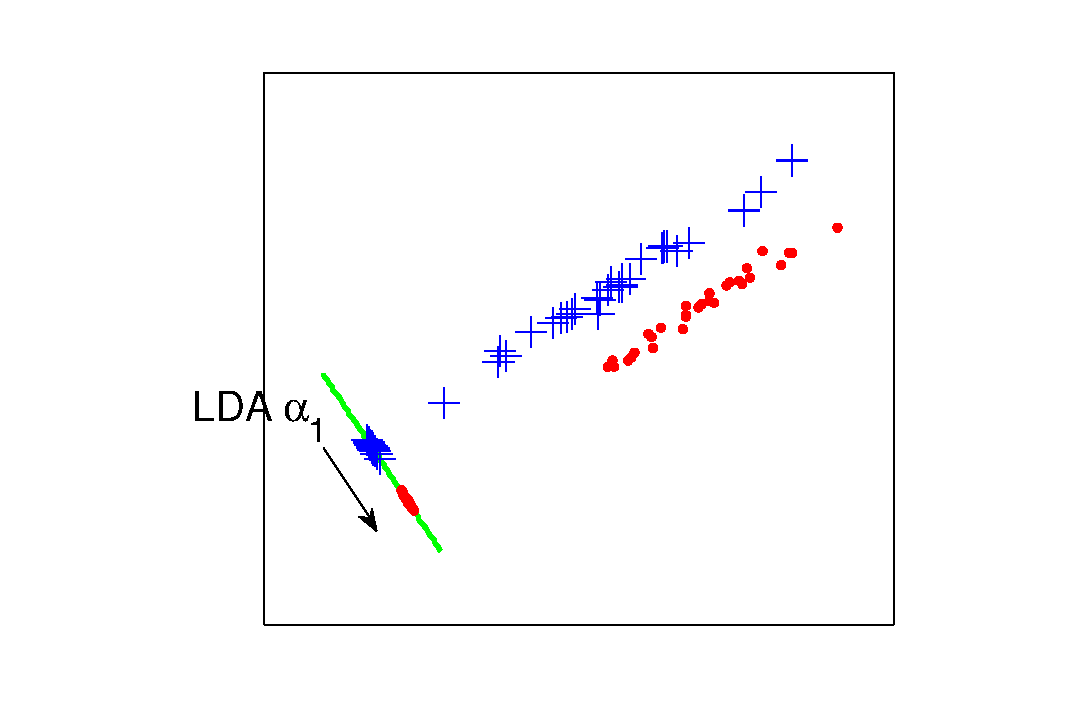
\includegraphics[width=\textwidth]{figures/LDAprojection.pdf} 
\end{column}
\begin{column}{.6\linewidth}
\begin{itemize}
\item LDA: linear decision boundary $a = \vec{w}^\intercal \vLeakVec + w_0$
\item Equivalently, project data onto $\vec{w}^\intercal \vLeakVec$ (orthogonally to the decision boudary), than classify by a real threshold (optimally $w_0$). \\
\end{itemize}
\end{column}
\end{columns}

\begin{itemize}
\item Two assumptions about class-conditional densities: 
\begin{itemize}
\item Gaussian distributions with parameters $\mu_j, \Sigma_j$
\item Homoscedasticity: $\Sigma_j=\Sigma$ for all $j$
\end{itemize}
\end{itemize}

\begin{block}{Fact, abuse and preference for the dimensionality reduction formulation}
\begin{itemize}
\item When LDA assumptions are met, the solution of the Fisher's criterion coincides with $\vec{w}$. 
\item assumption not required
\item naturally multi-class
\end{itemize}
\end{block}

\end{frame}

\begin{frame}
\frametitle{Linear separability}
LDA: linear decision boundary $a = \vec{w}^\intercal \vLeakVec + w_0$ ($\vec{w} = \Sigma^{-1}(\mu_1-\mu_2)$)
%
\begin{block}{}
\begin{huge}
\centering What if $\mu_1 = \mu_2$? 
\end{huge}
\end{block}
\only<2->{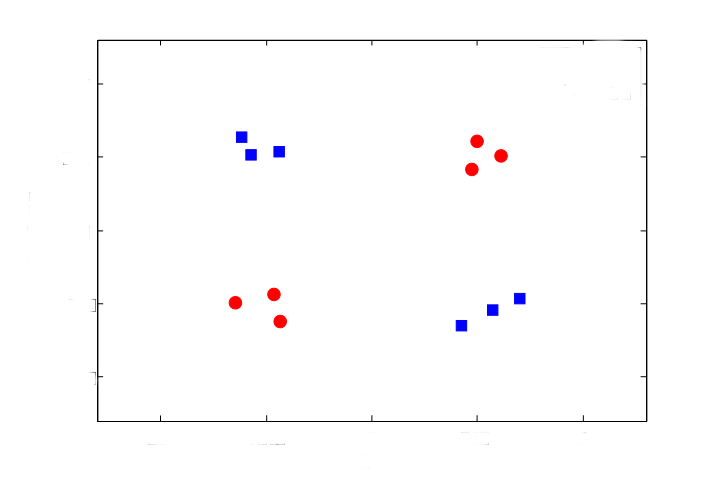
\includegraphics[width=.4\textwidth]{figures/D2.png} }
\only<3>{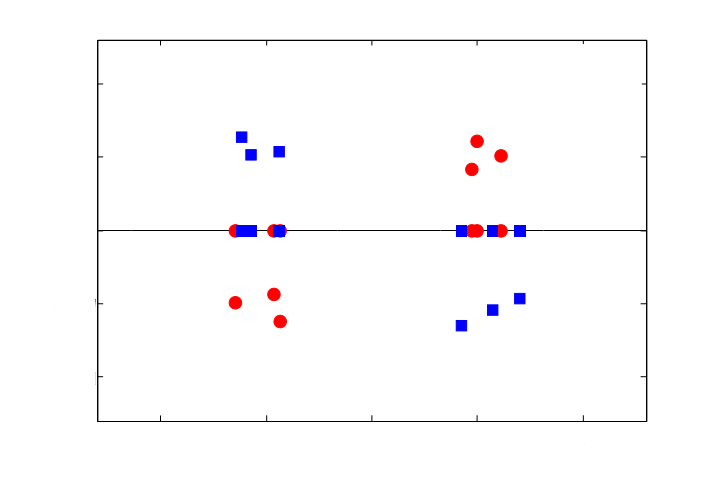
\includegraphics[width=.4\textwidth]{figures/D2_useless1.png} }
\only<4>{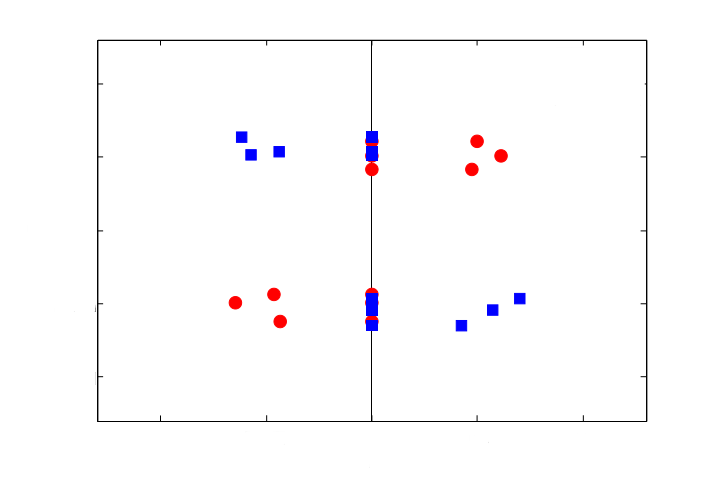
\includegraphics[width=.4\textwidth]{figures/D2_useless2.png} }
\only<5>{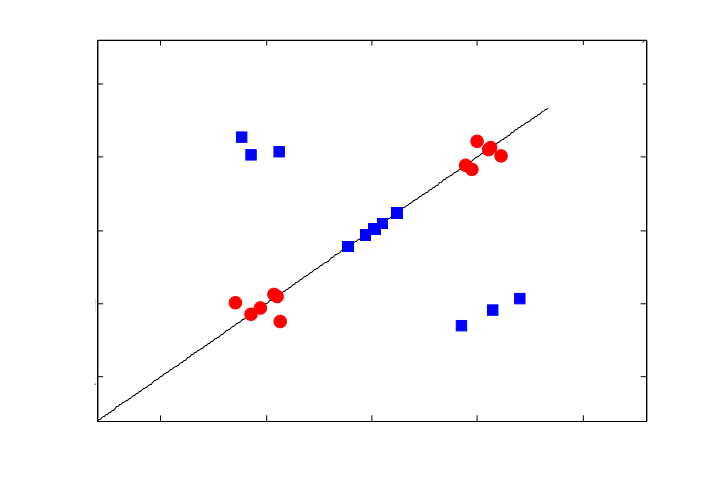
\includegraphics[width=.4\textwidth]{figures/D2_useless3.png} }
\only<6>{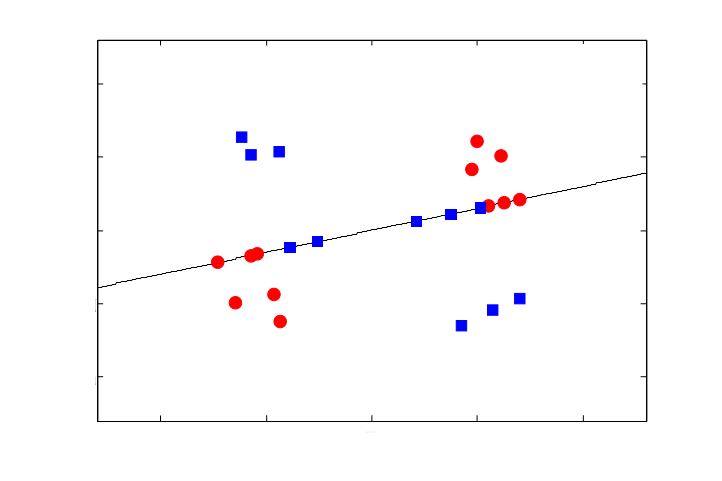
\includegraphics[width=.4\textwidth]{figures/D2_useless4.png} }
\end{frame}


\begin{frame}
\frametitle{Dimensionality reduction in presence of masking}
\begin{block}{$(d-1)$th-order Sharing (or Masking)} 
Split each sensitive $Z$ into shares  $Z = M_1 \star \dots \star M_d$ \\
with \only<1>{\textcolor{black}{$M_1, \dots , M_{d-1}$}}\only<2->{\textcolor{red}{$M_1, \dots , M_{d-1}$}} random shares (or masks) \only<2->{\textcolor{red}{UNKNOWN}} \\ and $M_d = Z \star M_1^{-1}\star \dots \star M_{d-1}^{-1}$ \\
Software implementations: shares are handled at different time samples $$t_1,\dots, t_d \qquad \only<1>{\mbox{\textcolor{white}{UNKNOWN}}} \only<2->{\mbox{\textcolor{red}{UNKNOWN}}} $$\\
$\Rightarrow$ each time sample is independent from $Z$.\\
\end{block}
\begin{columns}
\begin{column}{.5\textwidth}
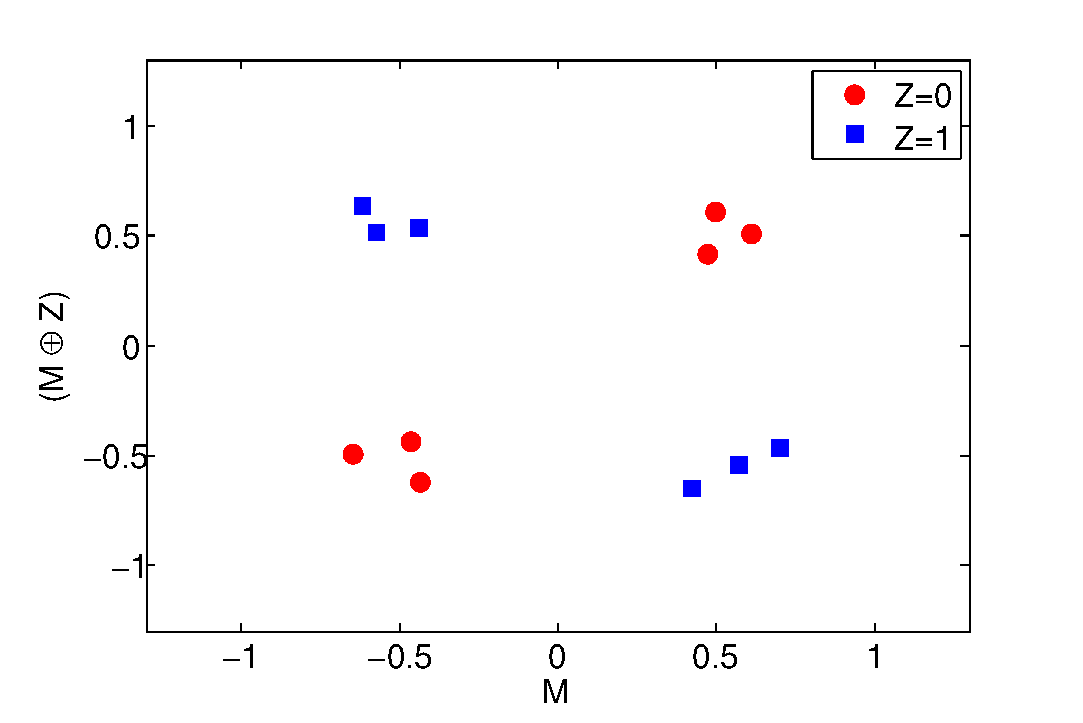
\includegraphics[\textwidth]{figures/D2.pdf}
\end{column}
\begin{column}{.5\textwidth}
\begin{block}{}
Toy example: 2 time samples, 1-bit data
\begin{itemize}
\item[$t_1$:] $M + n$, $n\sim \mathcal{N}(0,0.1)$ 
\item[$t_2$:] $M\oplus Z + n$ (Boolean masking)
\end{itemize}
\end{block}
\end{column}
\end{columns}



\end{frame}
\begin{frame}
\frametitle{In high-dimensional traces}
$f(z) = \esper[\vaLeakVec\lvert Z=z]$ is constant $\Rightarrow$ SNR, SOD, t-statistic are null!
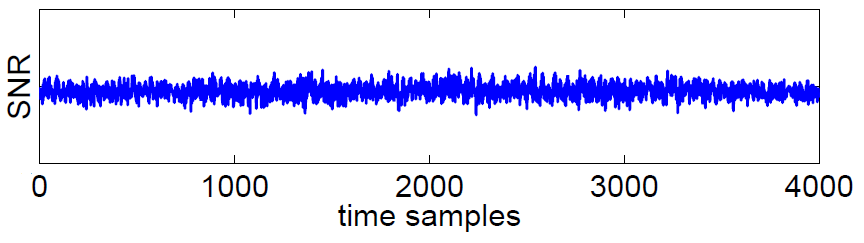
\includegraphics[width = 0.9\textwidth]{figures/SNR_2order_new.png} 
\pause
$\esper[A\vaLeakVec\lvert Z=z]$ is constant as well $\Rightarrow$ Projecting extractors can't help! 

\begin{block}{Higher-Order Side-Channel Attacks}
Exploit $f(z) = \esper\left[\vaLeakVec[t_1]\vaLeakVec[t_2]\dots\vaLeakVec[t_d]\lvert Z=z\right]$ non-constant.
 \end{block}

\begin{block}{Necessary condition}
\cite{carlet2014achieving} The statistic extracted from measurements must contain  $$\vaLeakVec[t_1]\vaLeakVec[t_2]\dots\vaLeakVec[t_d]$$
\end{block} 
\end{frame}

\begin{frame}
\frametitle{PoIs Research}
How to detect the $d$-tuple $t_1,\dots, t_d$? 
\begin{block}{A lacking literature}
\begin{itemize}
\item many HO attacks papers assume the knowledge of $t_1,\dots, t_d$
\item PoI research exploiting the random shares knowledge (back to unprotected case using $M_1,\dots , M_d$ instead of $Z$)
\item naive strategy: infer over all possible $d$-tuples 
\item Hand selection via educated guess \cite{Oswald2006}
\end{itemize}
\end{block}

\begin{block}{Generalizing extractors for higher-order context}
\begin{itemize}
\item Selecting extractors $\longrightarrow$ Projection Pursuits \cite{PP}
\item Projecting extractors $\longrightarrow$ Kernel Discriminant Analysis [CARDIS '16]
\end{itemize}
\end{block}
\end{frame}

\subsection{Kernel Discriminant Analysis}

\begin{frame}
[fragile]
\frametitle{KDA: the purpose}

\begin{block}{Problem}
Useful statistics lie in a high-dimensional \emph{feature} space: 
$$\featureSpace = \mathbb{R}^{{D+d-1}\choose{d}}$$
(all $d$th-degree monomials in the trace coordinates)
\end{block}

\begin{figure}
\centering
{
\begin{tikzpicture}
\matrix (m) [matrix of math nodes, row sep=3em,
column sep=3em, text height=1.5ex, text depth=0.25ex]
{ \mathbb{R}^\traceLength & \featureSpace & \mathbb{R}^\newTraceLength \\};
\path[->]
(m-1-1) edge node[above] {$\Phi$} (m-1-2);
         %edge [bend left=30] (m-2-2)
         %edge [bend right=15] (m-2-2);
\path[->]
($(m-1-2.north east)-(0,0.1)$) edge node[above] {$\extract^{\mathrm{PCA}}$} ($(m-1-3.north west)-(0,0.1)$);
\path[->]
($(m-1-2.south east)+(0,0.15)$) edge node[below] {$\extract^{\mathrm{LDA}}$} ($(m-1-3.south west)+(0,0.15)$);

\path[->]
(m-1-1) edge [bend left=50] node[above] {$\extract^{\mathrm{KPCA}}$} (m-1-3)
(m-1-1) edge [bend right=50] node[below] {$\extract^{\mathrm{KDA}}$} (m-1-3);

\node[text width=4cm] at (4,0) {\begin{footnotesize}
$\Phi$ non-linear function
\end{footnotesize}};
\end{tikzpicture} 
}


\end{figure}

\begin{block}{What KDA provides}
KDA allows performing LDA in $\featureSpace$, remaining in $\mathbb{R}^{D}$.
\end{block}

\end{frame}



\begin{frame}
%[fragile]
\frametitle{KDA: an intuition}
%\vspace{-30pt}
%\begin{figure}
%\centering
%{
%\begin{tikzpicture}
%\matrix (m) [matrix of math nodes, row sep=3em,
%column sep=3em, text height=1.5ex, text depth=0.25ex]
%{ \mathbb{R}^\traceLength & \featureSpace & \mathbb{R}^\newTraceLength \\};
%\path[->]
%(m-1-1) edge node[above] {$\Phi$} (m-1-2);
%         %edge [bend left=30] (m-2-2)
%         %edge [bend right=15] (m-2-2);
%\path[->]
%($(m-1-2.north east)-(0,0.1)$) edge node[above] {$\extract^{\mathrm{PCA}}$} ($(m-1-3.north west)-(0,0.1)$);
%\path[->]
%($(m-1-2.south east)+(0,0.15)$) edge node[below] {$\extract^{\mathrm{LDA}}$} ($(m-1-3.south west)+(0,0.15)$);
%
%\path[->]
%(m-1-1) edge [bend left=50] node[above] {$\extract^{\mathrm{KPCA}}$} (m-1-3)
%(m-1-1) edge [bend right=50] node[below] {$\extract^{\mathrm{KDA}}$} (m-1-3);
%
%\node[text width=4cm] at (4,0) {\begin{footnotesize}
%$\Phi$ non-linear function: all $d$th-degree monomials of time samples
%\end{footnotesize}};
%\end{tikzpicture} 
%}
%
%
%\end{figure}
\vspace{-15pt}
\begin{block}{}
Toy example: 2 time samples, 1-bit data
\begin{itemize}
\item[$t_1$:] $M + n$, $n\sim \mathcal{N}(0,0.1)$ 
\item[$t_2$:] $M\oplus Z + n$ (Boolean masking)
\end{itemize}
\end{block}

\begin{columns}
\begin{column}{.5\textwidth}
\uncover<1->{
\only<1-3>{
\begin{figure}
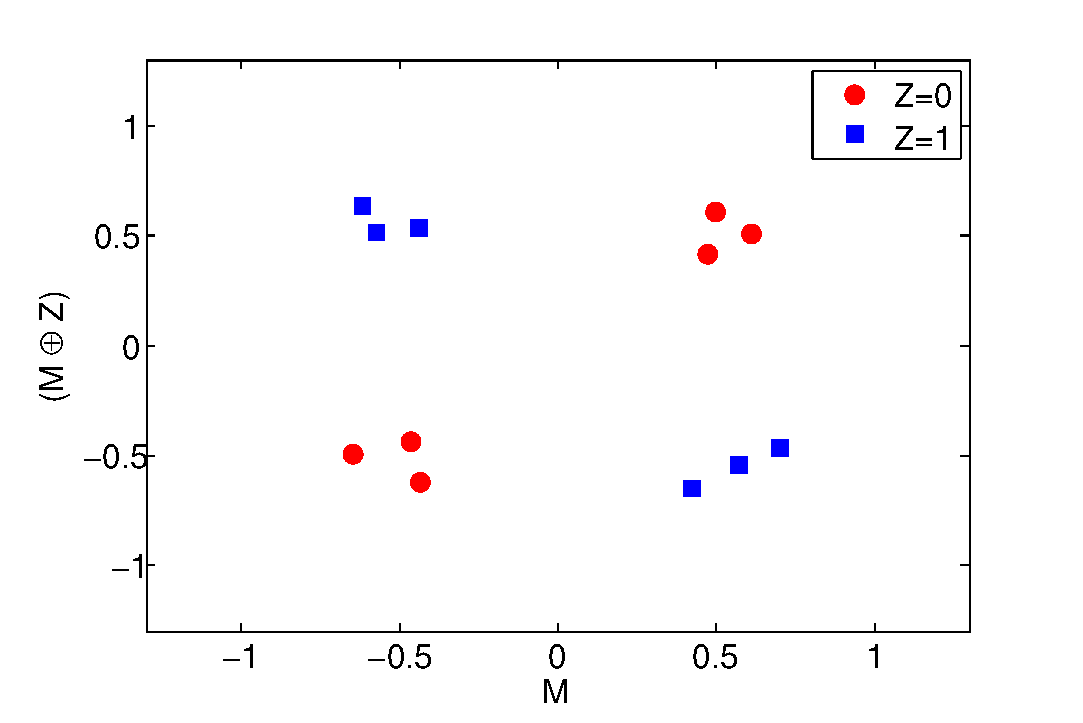
\includegraphics[width=\textwidth]{figures/D2.pdf}
\end{figure}}

\only<4>{
\begin{figure}
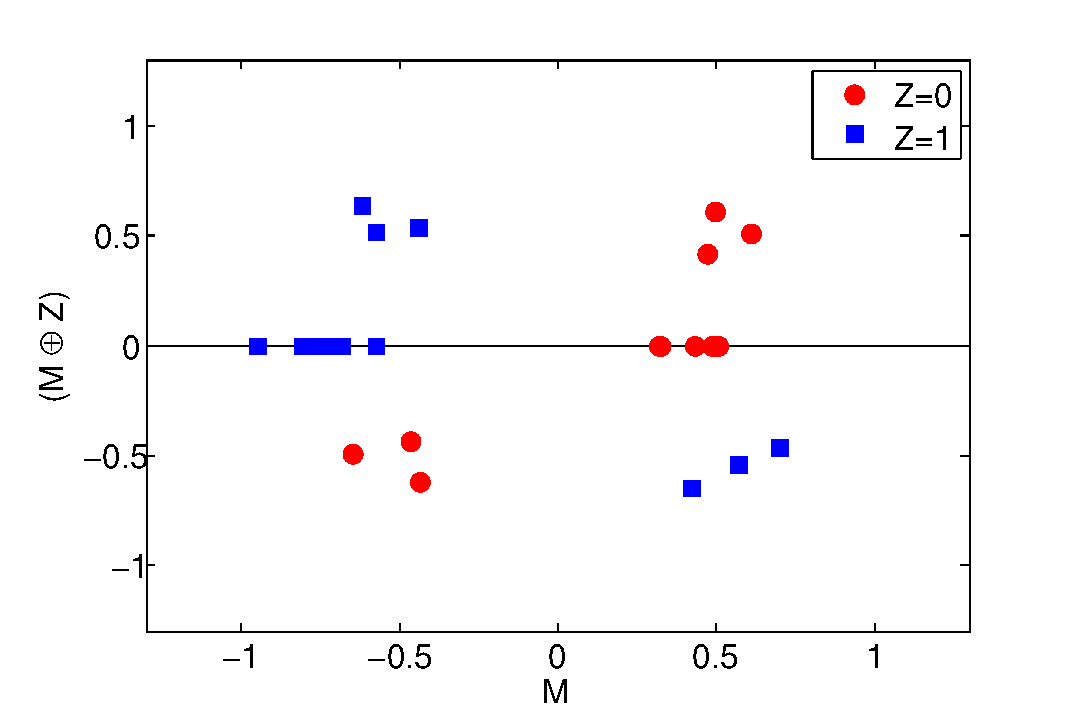
\includegraphics[width=\textwidth]{figures/D2_proj.pdf}
\end{figure}
\centering
\textcolor{violet}{\Large{KDA} \\ \large{remains in $\mathbb{R}^D$}}
}
\only<5->{
\begin{figure}
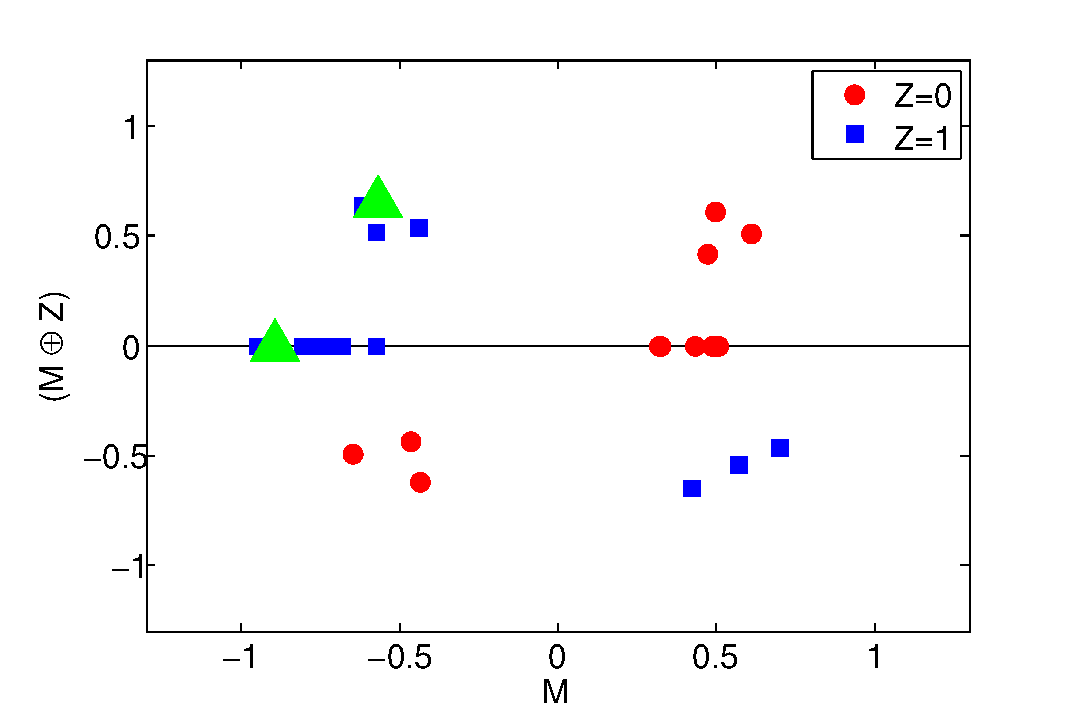
\includegraphics[width=\textwidth]{figures/new_example_KDA.pdf} 
\end{figure}}
}

\end{column}

\begin{column}{.5\textwidth}
\uncover<2->{
\only<1-2>{
\begin{figure}
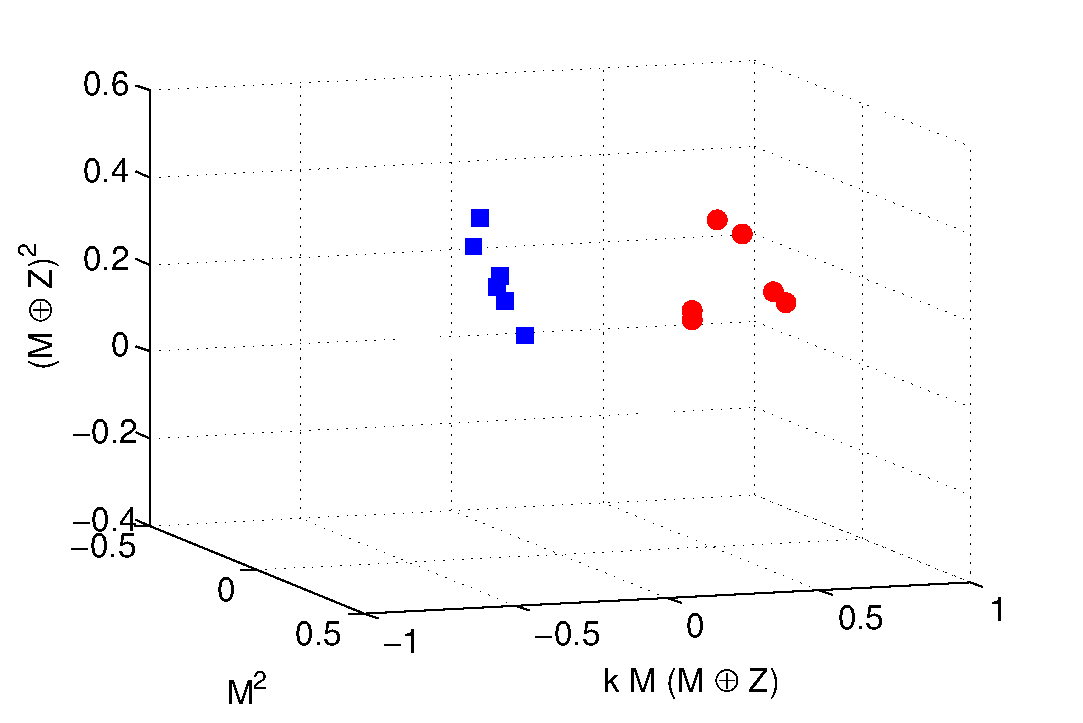
\includegraphics[width=\textwidth]{figures/D3.pdf} 
\end{figure}
\centering
\textcolor{violet}{\Large{ $\Phi\colon \mathbb{R}^D \rightarrow \mathbb{R}^{{D+d-1}\choose{d}}$  \\ $\Phi(t_1,t2) = (t_1^2, t_2^2, kt_1t_2)$ }}
}
\only<3>{
\begin{figure}
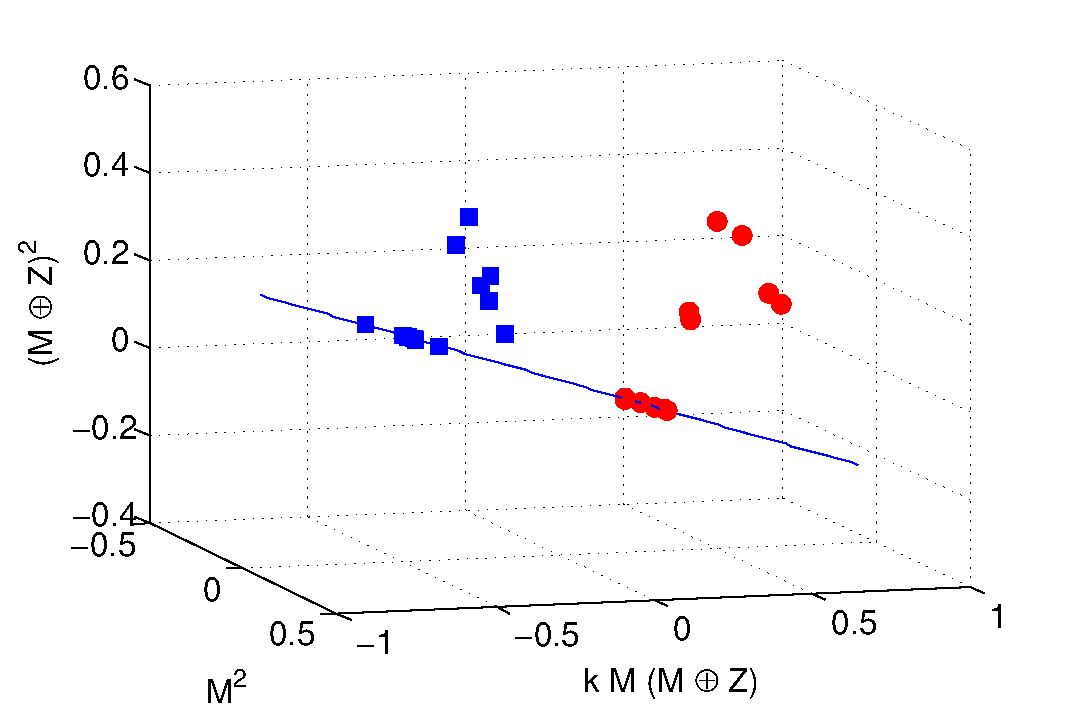
\includegraphics[width=\textwidth]{figures/D3_proj.pdf} 
\end{figure}
\centering
\textcolor{violet}{\Large{$\Phi \longrightarrow$ LDA}}
}
\only<4>{
\begin{figure}
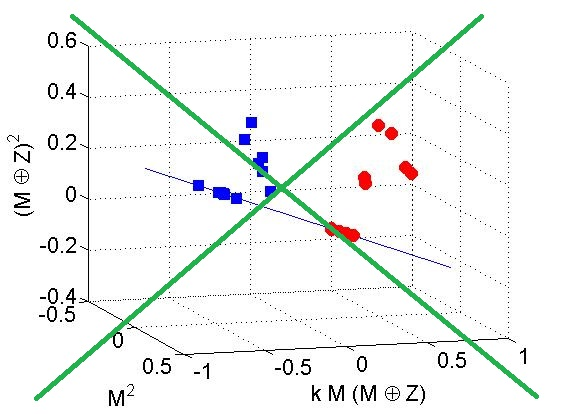
\includegraphics[width=\textwidth]{figures/D3_proj.jpg} 
\end{figure}
}}

\only<5->{
\begin{block}{KDA procedure}
\begin{itemize}
\item Training $\rightarrow \textcolor{violet}{\boldsymbol{\nu}_\ell}$ , $C$ vectors of coefficients ($\ell = 1,\dots , C$)
\item<6-> \emph{Compare} the new trace with all training traces $K(\textcolor{red}{\sss[z_i]{i}}, \textcolor{green}{\sss[]{}})$, $K(\textcolor{blue}{\sss[z_i]{i}}, \textcolor{green}{\sss[]{}})$
\item<7-> \emph{KDA projection} \begin{equation}\label{eq:projection}
\extract^{\mathrm{KDA}}_{\ell}(\vec{x}) = \sum_{i=1}^{\NPoI}\textcolor{violet}{\boldsymbol{\nu}_\ell[i]}K(\sss[z_i]{i}, \textcolor{green}{\sss[]{}}) \mbox{ .}
\end{equation} 
\end{itemize}

\end{block}
}

\end{column}
\end{columns}
%\uncover<5>{
%\begin{block}{Apply KDA extractor}
%\begin{equation}\label{eq:projection}
%\extract^{\mathrm{KDA}}_{\ell}(\vec{x}) = \sum_{i=1}^{\NPoI}\boldsymbol{\nu}_\ell[i]K(\textcolor{red}{\sss[z_i]{i}}, \textcolor{green}{\sss[]{}}) \mbox{ .}
%\end{equation} 
%
%
%\end{block}
%}
\end{frame}


\begin{frame}
\frametitle{Kernel Function}

\begin{block}{Kernel Function}
$K\colon\mathbb{R}^D\times \mathbb{R}^D \rightarrow \mathbb{R} \nonumber$
\begin{equation}\label{eq:kernelProperty}
K(\sss[]{i},\sss[]{j}) = \Phi(\sss[]{i})\cdot \Phi(\sss[]{j})
\end{equation}
\end{block}

\begin{block}{Polynomial Kernel Function}
$K(\sss[]{i},\sss[]{j}) = (\sss[]{i} \cdot \sss[]{j})^d \qquad \leftrightarrow \qquad\Phi:\mathbb{R}^D \rightarrow \mathcal{F}\subset \mathbb{R}^{{D+d-1}\choose{d}} $ all $d$th-degree monomials


\end{block}
\uncover<2->{
\begin{block}{Example: $2$nd Degree Polynomial Kernel Function}
Toy example: $D=2 \longrightarrow \sss[]{i} = [a,b]$ , $\sss[]{j} = [c,d]$
\begin{equation*}
K(\sss[]{i},\sss[]{j}) = (ac + bd)^2 = a^2c^2 + 2abcd + b^2d^2
\end{equation*}
\only<2>{
\textcolor{white}{$K \longleftrightarrow$ $\Phi\colon \Bbb{R}^2\rightarrow\Bbb{R}^3$
\begin{equation*}
\Phi(u,v) =  [u^2, \sqrt{2}uv, v^2]
\end{equation*}}
}
\uncover<3->{
$K \longleftrightarrow$ $\Phi\colon \Bbb{R}^2\rightarrow\Bbb{R}^3$
%\begin{align}
%&\Phi \colon \mathbb{R}^2 \rightarrow \mathbb{R}^3\\
%&\Phi \colon [a,b]\mapsto [a^2, \sqrt{2}ab, b^2]\\
%&\Phi \colon [c,d]\mapsto [c^2, \sqrt{2}cd, d^2].
%\end{align}
\vspace{-5pt}
\only<3>{
\begin{equation*}
\Phi(u,v) =  [u^2, \sqrt{2}uv, v^2]
\end{equation*}}
\only<4>{
\begin{equation*}
\Phi(a,b) =  \textcolor{magenta}{[a^2, \sqrt{2}ab, b^2]}
\end{equation*}
}
\only<5>{
\begin{equation*}
\Phi(c,d) =  \textcolor{blue}{[c^2, \sqrt{2}cd, d^2]}
\end{equation*}
}
}

\only<3>{
\textcolor{white}{$\Phi(\sss[]{i})\cdot \Phi(\sss[]{j}) = {a^2}{c^2} + {\sqrt{2}ab}{\sqrt{2}cd} + {b^2}{d^2} = K(\sss[]{i},\sss[]{j})$}}

\only<4>{
$\Phi(\sss[]{i})\cdot \Phi(\sss[]{j}) = \textcolor{magenta}{a^2}\textcolor{white}{c^2} + \textcolor{magenta}{\sqrt{2}ab}\textcolor{white}{\sqrt{2}cd} + \textcolor{magenta}{b^2}\textcolor{white}{d^2} = K(\sss[]{i},\sss[]{j})$}

\only<5>{
$\Phi(\sss[]{i})\cdot \Phi(\sss[]{j}) = \textcolor{magenta}{a^2}\textcolor{blue}{c^2} + \textcolor{magenta}{\sqrt{2}ab}\textcolor{blue}{\sqrt{2}cd} + \textcolor{magenta}{b^2}\textcolor{blue}{d^2} = K(\sss[]{i},\sss[]{j})$}

\end{block}
}

\end{frame}



\begin{frame}

\frametitle{KDA - the training}
\begin{center}
\only<1>{
Between-class (inter-class) Scatter Matrix }
\only<2>{
Within-class (inter-class) Scatter Matrix }
\only<3>{
Eigenvector problem}
\only<4>{
New trace projection}

\end{center}

\begin{columns}
\begin{column}{.5\textwidth}
\uncover<3->{Computational Complexity $O(D^3)$}
\begin{block}{LDA}
\begin{small}
\begin{itemize}
\item $\SB = \sum_{\sensVar\in\sensVarSet}\numTraces(\mmmXclass-\mmmX)(\mmmXclass-\mmmX)^\intercal$ 
\uncover<2->{\item $\SW = \sum_{\sensVar\in\sensVarSet}\sum_{i=1}^{\numTraces}(\sss{i}-\mmmXclass)(\sss{i}-\mmmXclass)^\intercal$ }
\uncover<3->{\item $\AAlpha_i$ eigenvectors of $\SW^{-1}\SB$ [$D\times D$]}
\uncover<4->{\item $\extract^{LDA}_{\ell}(\xxx) = \sum_{i=1}^D \AAlpha_{\ell}[i]\xxx[i] $}
\end{itemize}
\end{small}
\end{block}
\end{column}

\begin{column}{.55\textwidth}
\uncover<3->{Computational Complexity $O(N^3)$}
\begin{block}{KDA}
\begin{small}
\begin{itemize}

\item $\MMM = \sum_{\sensVar\in\sensVarSet}\numTraces(\MMMclass - \MMMT)(\MMMclass-\MMMT)^\intercal$ \footnotemark

\uncover<2->{\item $\NNN = \sum_{\sensVar\in\sensVarSet}\kernelMatrix_\sensVar(\III - \III_{\numTraces})\kernelMatrix_\sensVar^\intercal$ \only<2-4>{\footnotemark} \only<5>{ \textcolor{red}{$+ \mu\III$}}}

\uncover<3->{\item $\nununu_i$ eigenvectors of $\NNN^{-1}\MMM$ [$N\times N$]}
\uncover<4->{\item $\extract^{\mathrm{KDA}}_{\ell}(\vec{x}) = \sum_{i=1}^{\NPoI}\nununu_\ell[i]K(\sss[z_i]{i}, \sss[]{}) $}
\end{itemize}
\end{small}
\end{block}
\end{column}
\end{columns}
\centering
\vspace{8pt}
\only<5>{\textcolor{red}{$\mu$ regularization parameter}}

\footnotetext[1]{$\MMMclass$ and $\MMMT$ are two $N$-sized column vectors whose entries are given by: $\MMMclass[z][j] = \frac{1}{\numTraces}\sum_{i:z_i=z}^{\numTraces}K(\sss[z_j]{j},\sss[z_i]{i}), \qquad
\MMMT[j] = \frac{1}{\NPoI}\sum_{i=1}^{\NPoI}K(\sss[z_j]{j},\sss[z_i]{i}) \mbox{ .}$}

\uncover<2->{\footnotetext[2]{$\III$ is a $\numTraces\times \numTraces$ identity matrix, $\III_{\numTraces}$ is a $\numTraces\times \numTraces$ matrix with all entries equal to $\frac{1}{\numTraces}$ and $\kernelMatrix_{\sensVar}$ is the $\NPoI\times \numTraces$ sub-matrix of $\kernelMatrix = (K(\sss[z_i]{i},\sss[z_j]{j}))_{\substack{i=1,\dots,\numTraces[] \\ j=1,\dots,\numTraces[]}}$ storing only columns indexed by the indices $i$ such that $z_i=z$}}
\end{frame}


\subsection{Experimental Results}


\begin{frame}
\frametitle{Experimental results}
\begin{itemize}
\item $D = 200$: length of rough trace (interesting clock cycles selected)
\item $d=2$, feature extracted from a $200^2 = 40.000$-sized space
\item $d=3 \rightarrow 200^3=6.000.000$ , $d=4 \rightarrow 200^4 = 800.000.000$
\end{itemize}
\begin{figure}[t]

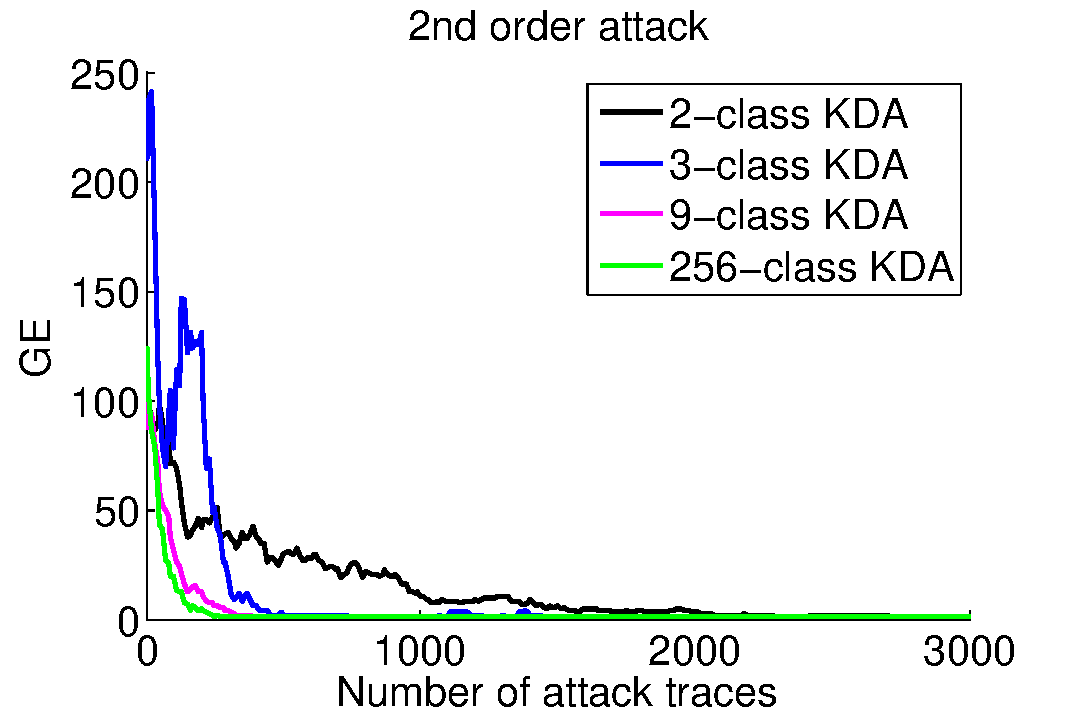
\includegraphics[width=.4\textwidth]{../Figures/CARDIS2016/2order_classes_TA.pdf}
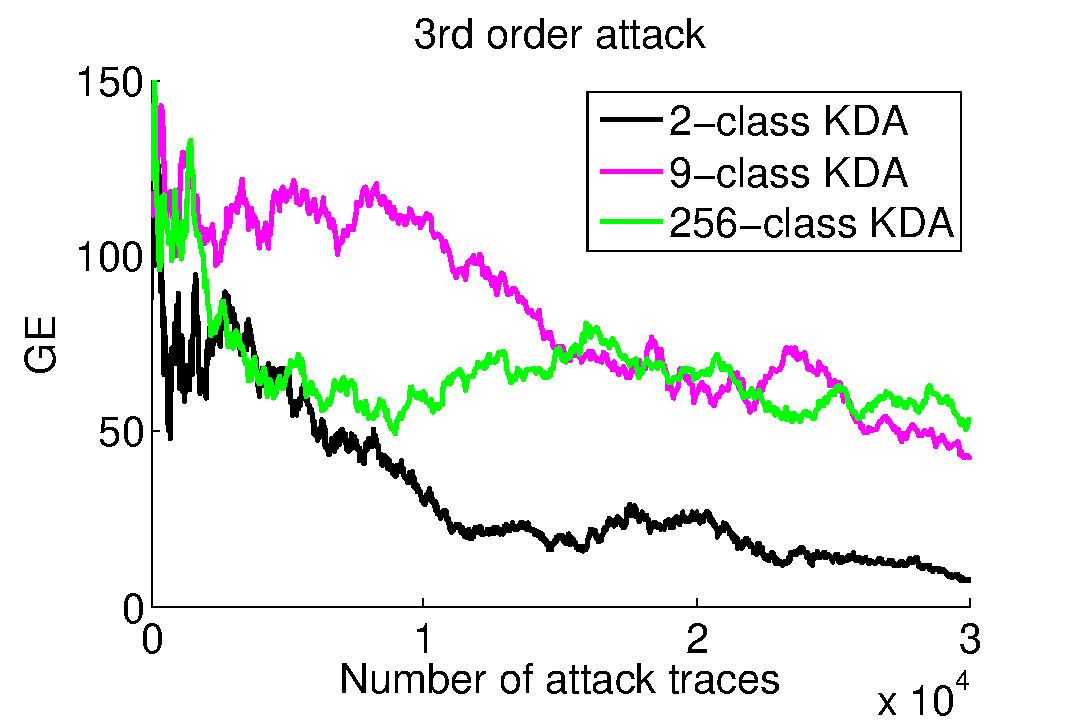
\includegraphics[width=.4\textwidth]{../Figures/CARDIS2016/3order_new.pdf}
\end{figure}
\vspace{-10pt}
\begin{figure}[t]

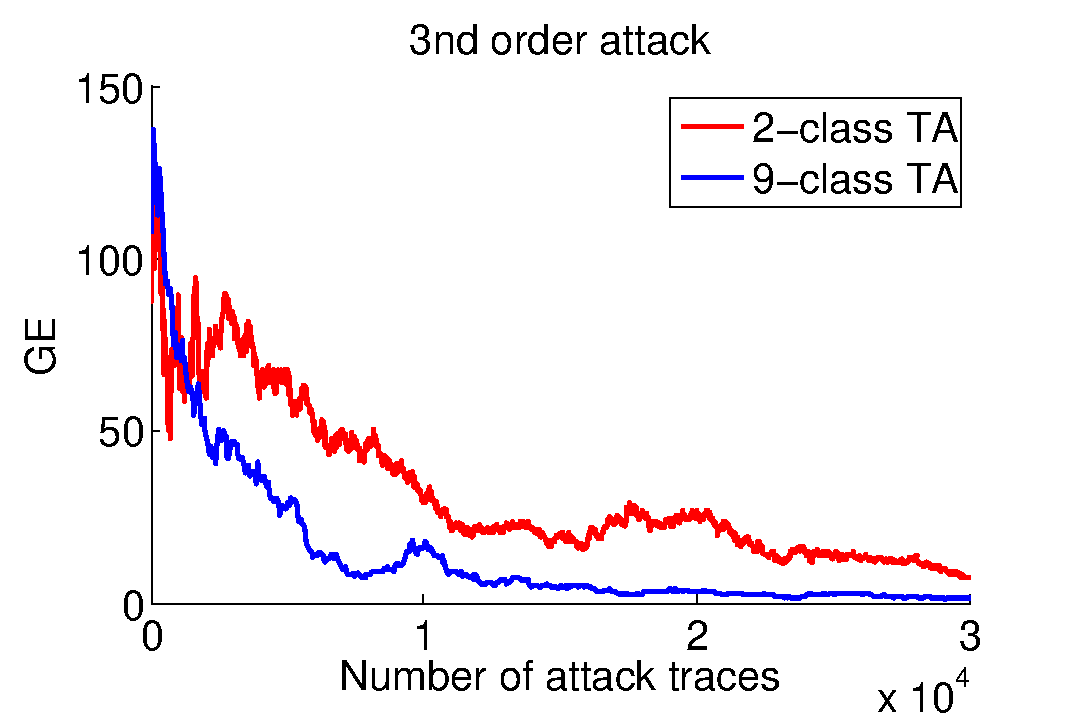
\includegraphics[width=.4\textwidth]{../Figures/CARDIS2016/3order_2_9.pdf}
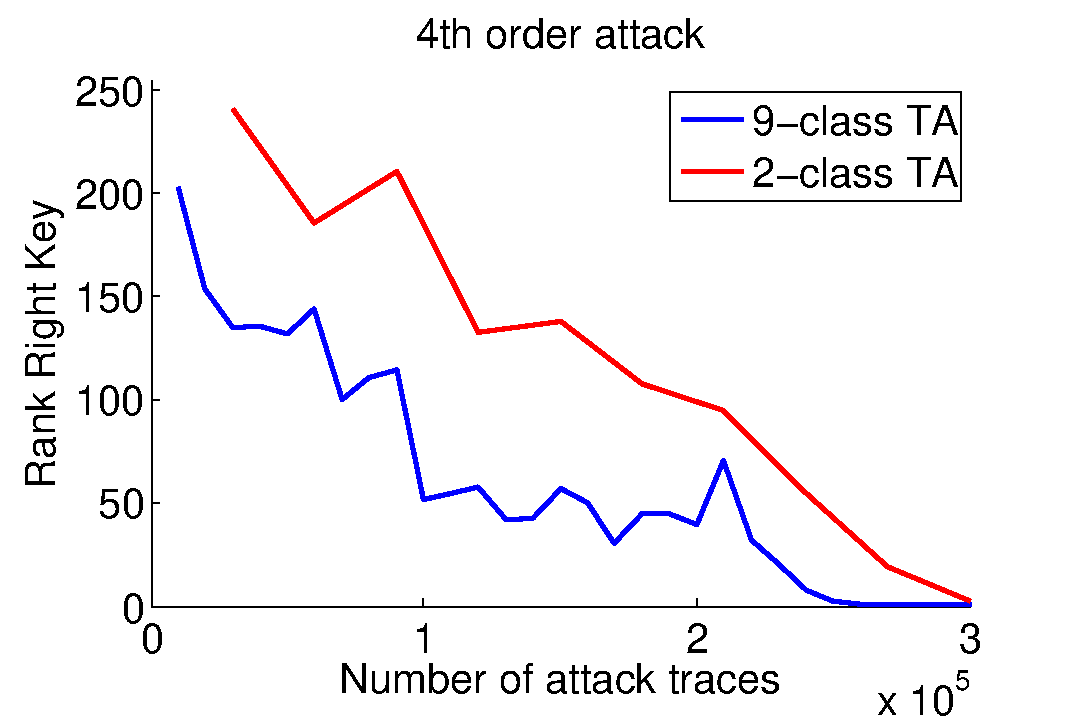
\includegraphics[width=.4\textwidth]{../Figures/CARDIS2016/4order_2_9.pdf}
\end{figure}
\end{frame}

\begin{frame}
\frametitle{Limits and Drawbacks}

\end{frame}